\section{Conclusiones}
\begin{frame}
	\frametitle{Conclusiones}
	\begin{figure}
	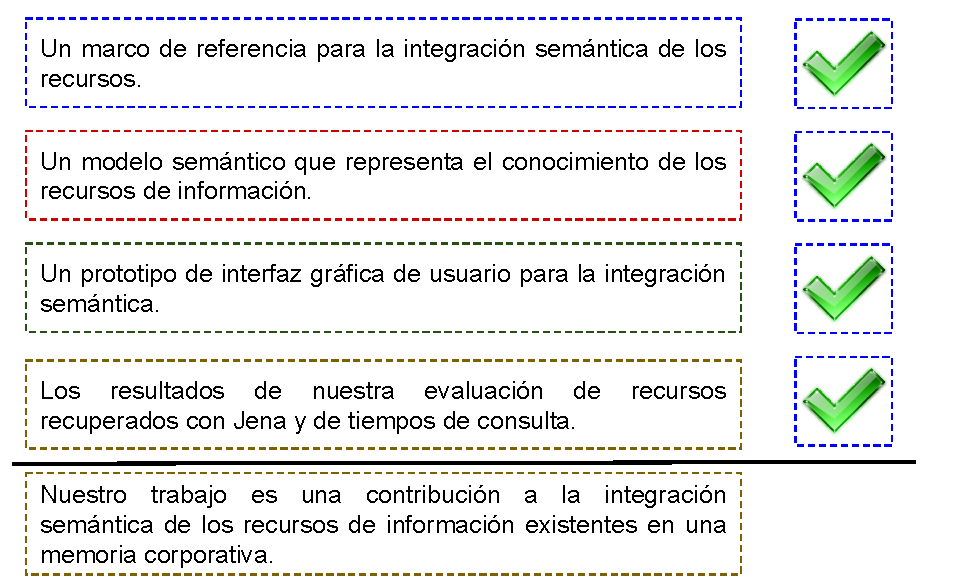
\includegraphics[scale=0.6]{ConclusionesObj} 
	\end{figure}
\end{frame}

\begin{frame}
	\frametitle{Conclusiones}
	\begin{exampleblock}{Hip�tesis}
	\justifying 
	\textbf{El uso de las \textit{tecnolog�as sem�nticas} es adecuado para lograr la \textit{integraci�n sem�ntica} de \textit{recursos de informaci�n} en una \textit{memoria corporativa}}.
	\end{exampleblock}
	
	\begin{block}{Ventajas de las Tecnolog�as Sem�nticas}
	\begin{itemize}[<+-| alert@+>]
%	\item \justifying Modelos en un formato est�ndar.
	\item \justifying Modelos flexibles, extensibles y reutilizables.
	\item \justifying Uso de Lenguajes est�ndar (World Wide Web Consortium).
	\item \justifying Modelos con conocimiento expl�cito e impl�cito.
	\item \justifying Inferencia para materializar tripletas RDF.
	\item \justifying Aplicaciones gen�ricas.
	\end{itemize}
	\end{block}
\end{frame}

\begin{frame}
	\frametitle{Recomendaciones}
	\begin{block}{}
	\begin{itemize}[<+-| alert@+>]
	\item \justifying Introducir nuevos \textit{casos de uso} para modelar mayor conocimiento del �rea de \textit{Redes y Telecomunicaciones}.
	\item \justifying Mejorar la seguridad del prototipo y agregar un recuadro para b�squedas por \textit{palabras clave}.
	\item \justifying Construir un modulo (aplicaci�n) para generar \textit{tripletas RDF} a partir de las descripciones de los \textit{recursos de informaci�n}.
		\begin{itemize}
		\item \justifying \small Generaci�n guiada por los usuarios.
		\item \justifying \small Generaci�n automatizada.
		\end{itemize}
%	\item \justifying Construir un modulo para visualizar y manipular \textit{tripletas RDF} del conocimiento expl�cito en una \textit{ontolog�a}.
	\item \justifying Comparar los tiempos de procesamiento y recursos relevantes con otros triplestores: \textit{Stardog} y \textit{Sesame}.
%	\item \justifying Traducir la ontolog�a a otros idiomas: \textit{espa�ol}, \textit{franc�s}, \textit{alem�n}, entre otros.
	\end{itemize}	
	\end{block}
\end{frame}